\subsection{Εξαγωγή δεδομένων}

Για την επεξεργασία των αποτελεσμάτων του ερωτηματολογίου και την καλύτερη κατανόησή τους, υλοποιήθηκε ένα \gls{script} σε Python. Το \gls{script} αυτό ενώνει τα δεδομένα για τους διαφορετικούς αλγόριθμους, ώστε να είναι πιο κατανοητά συνολικά, και υπολογίζει το σκορ \acrshort{sus}.

\begin{figure}[H]
    \centering
    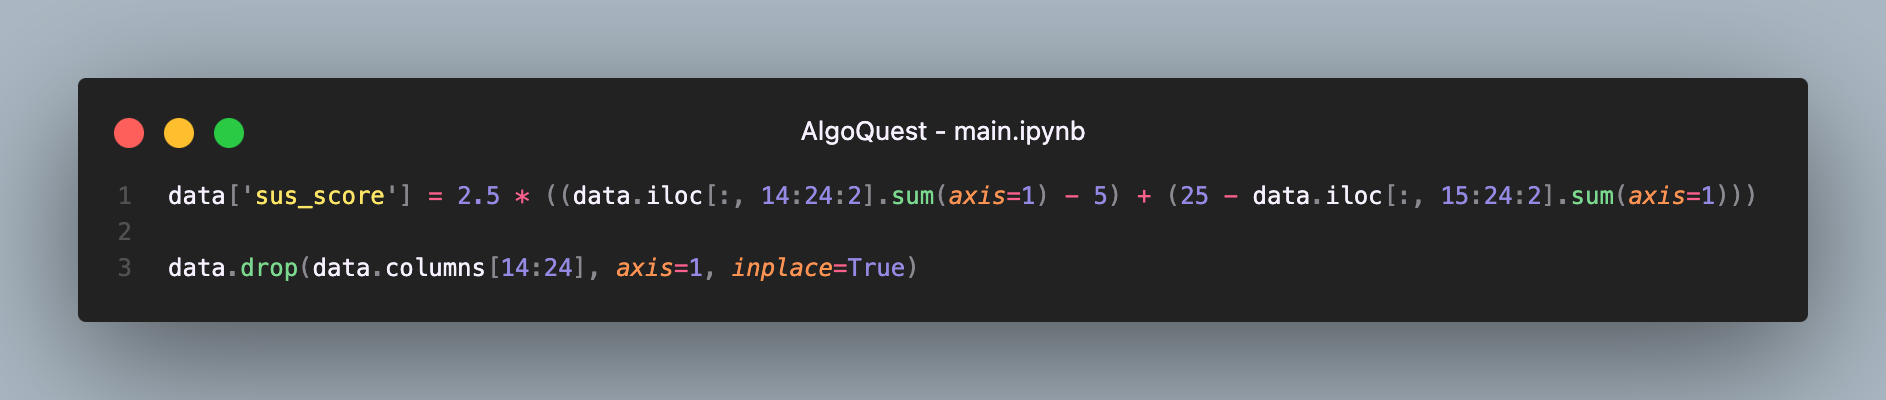
\includegraphics[width=1\linewidth]{sections/5/3/images/sus_score_calculation}
    \caption{Υπολογισμός σκορ \acrshort{sus}}
    \label{fig:sus_score_calculation}
\end{figure}

Το \gls{script} δέχεται ως είσοδο τα αποτελέσματα του ερωτηματολογίου σε μορφή \acrshort{csv} και εξάγει τα ζητούμενα αποτελέσματα. Μπορεί εύκολα να χρησιμοποιηθεί στο μέλλον για την επεξεργασία επιπλέον δεδομένων από το ερωτηματολόγιο.
